\documentclass[a4paper,oneside,frenchb,10pt]{article}

\usepackage[T1]{fontenc}
\usepackage[utf8x]{inputenc}
\usepackage{amsmath}
\usepackage{babel}
\usepackage{fancyhdr}
\usepackage{fourier}
\usepackage{fullpage}
\usepackage{graphicx}
\usepackage{hyperref}
\usepackage{listings}
\usepackage{textcomp}
\usepackage{url}

\hypersetup{colorlinks=true, linkcolor=black}

\pagestyle{plain}

\setcounter{tocdepth}{2}

\setlength{\parindent}{0pt}
\setlength{\parskip}{4pt plus 2pt minus 1pt}

\title{SynthLab\\Simulateur de Synthétiseur de son analogique}
\author{Cyrille \textsc{Folliot} : Responsable documentation, \\Julien \textsc{Névo} : Responsable projet,\\ Julien \textsc{Richard-Foy} : Responsable conception,\\ Maxime \textsc{Simon} : Responsable qualité.} 
 
\begin{document}
\maketitle
\tableofcontents

\section{Introduction}

Ce projet, baptisé \textbf{SynthPro}, consiste à réaliser une
application permettant de simuler numériquement les sons issus des
premiers synthétiseurs analogiques, dits à synthèse soustractive.

Le principe de l'application est basé sur la modularité~:
l'utilisateur doit pouvoir assembler des modules sonores entre eux
et entendre le résultat du montage en temps-réel. Il n'y a,
\emph{a priori}, pas de limitation quant au nombre de modules
pouvant être ajoutés, et la manière dont ils sont connectés doit
rester aussi permissive que possible.

\subsection{L'équipe}

\subsubsection{Présentation de l'équipe}

Notre équipe, portant le nom de \textbf{BackSynth Boys} (en
l'honneur d'un certain \emph{boys band}) est composée de quatre
personnes, chacune ayant un rôle particulier à remplir dans la
gestion du projet en lui-même, mais bien sûr également dans la
conception et la production de l'application~:

\begin{itemize}
\item
  Julien Richard-Foy~: \textbf{responsable Conception}. Chargé de la
  bonne conception et structuration du projet. S'est occupé de la
  partie Métier, de la communication entre celle-ci et l'interface
  graphique, et l'interface graphique en elle-même~;
\item
  Maxime Simon~: \textbf{reponsable Qualité}. Chargé de la bonne
  formation des programmes écrits, aussi bien structurellement que
  syntaxiquement, et de la pertinence des tests effectués. S'est
  également occupé de l'interface et de la communication avec la
  partie Métier~;
\item
  Julien Névo~: \textbf{responsable Projet}. Chargé de faire les
  rapports d'avancement du travail auprès de M. Plouzeau. S'est
  occupé du moteur audio, de la génération sonore des VCO et VCF, et
  de divers modules~;
\item
  Cyrille Folliot~: \textbf{responsable Documentation}. Chargé de la
  qualité de la documentation produite. S'est également attelé au
  développement des modules et de la partie Métier.
\end{itemize}
\subsubsection{Organisation du temps de travail}

Quatre semaines nous étaient imparties pour mener à bien ce projet.
Les trois premiers jours furent utilisés pour mettre en place
l'architecture du projet et la conception de la partie Métier. Une
fois cela fait, nous nous sommes répartis les rôles en fonction de
nos affinités pour le travail à effectuer. Le travail de chacun a
pu être fait de manière indépendante très rapidement.

Nous avons mis en place des \textbf{itérations}, très courtes, dans
lesquelles étaient consignées les tâches que chacun devait
accomplir. Le but étant qu'à la fin de chaque itération, le projet
fonctionne toujours et soit à chaque fois agrémenté de nouvelles
fonctionnalités. Une itération peut durer de 1 à 3 jours.

\subsubsection{Logiciels et outils de développement}

\paragraph{Outils de développement}

Notre projet est basé sur le \emph{framework} Qt, dans le langage
C++. Nous avons utilisé l'environnement fourni, QtCreator, qui
fonctionne aussi bien sous Linux et Windows. Notre utilisateur de
Mac~OS~X a utilisé Xcode.

\paragraph{Versionnement}

Nous avons choisi d'utiliser Git pour le versionnement de notre
application, et ce pour trois raisons~:

\begin{itemize}
\item
  SVN est connu de tous, et nous désirions utiliser un nouveau
  logiciel pour les comparer~;
\item
  Git s'avère plus efficace à gérer les conflits entre les différents
  \emph{commits} que SVN. Ce projet étant mené par 4 personnes, il
  était nécessaire de prévoir ce genre de situations~;
\item
  GitHub, une interface \emph{Web} de Git et liée au dépôt de
  fichiers, fut très pratique pour gérer le projet. Elle permet
  notamment de voir l'historique de chaque fichier, du projet en
  général, et du travail effectué par chaque personne.
\end{itemize}

\paragraph{Documentation}

Les schémas UML ont été mis en oeuvre sous BouML. La plupart des
documents ont été écrits dans le wiki de GitHub, puis convertis au
format LaTeX grâce à Pandoc.


%\section{Compte-rendu}

\begin{enumerate}[1.]
\item
  [[Compte-rendu : Introduction]]
\item
  Modèle Métier
  \begin{enumerate}[1.]
  \item
    Modules
  \item
    Entrées/Sorties
  \item
    Connexions et communications entre les modules (Buffer\ldots{})
  \end{enumerate}
\item
  [[Conception — PIM]]
  \begin{enumerate}[1.]
  \item
    PAC / Héritage
  \end{enumerate}
\item
  [[Conception — PSM]]
  \begin{enumerate}[1.]
  \item
    Choix technologiques
  \item
    Conséquences en terme d'architecture
    \begin{enumerate}[1.]
    \item
      L'héritage multiple
    \end{enumerate}
  \item
    Conséquences en terme d'implémentation
    \begin{enumerate}[1.]
    \item
      La gestion du son
    \item
      Un autre point
    \end{enumerate}
  \item
    Conséquences au niveau de la gestion de l'UI
  \end{enumerate}
\item
  [[Tests et Validation]]
  \begin{enumerate}[1.]
  \item
    Tests unitaires
  \end{enumerate}
\item
  Methode de travail
  \begin{enumerate}[1.]
  \item
    Les itérations (un peu d'agilité que diable)
  \item
    Le partage des responsabilités au niveau de l'équipe
  \item
    Conclusion sur les méthodes de travail
  \end{enumerate}
\end{enumerate}

\section{Modèle Métier}

\subsection{Le synthétiseur}

L'application que nous développons consiste à simuler numériquement
le comportement des synthétiseurs analogiques, dits à synthèse
soustractive, ainsi que l'aspect modulaire de leur utilisation.
Chaque synthétiseur est composé de \textbf{Modules} que l'on
pourra lier entre eux, tout en écoutant le résultat du
montage en temps-réel.

\subsection{L'interface}

L'application possède un environnement graphique qui permet à
l'utilisateur de visualiser l'intégralité des modules disponibles.
Il aura également à sa disposition une surface qu'il pourra remplir
à loisir en déposant des modules du type désiré. Les différents
paramètres des modules peuvent également être modifiables en
temps-réel.

\subsection{Les modules}

Le module est la partie atomique du montage. Il n'existe pas \emph{a
priori} de limite au nombre de modules que l'on peut créer. Un
module dispose d'au moins une entrée et/ou une sortie. Certains
modules, sources de flux, ne disposent pas d'entrée, comme les
oscillateurs dont le but est de générer des ondes. D'autres, appelés
\emph{puits}, n'ont pas de sortie et sont utiles en fin de
montage pour, par exemple, diriger le son vers une sortie audio ou
afficher le résultat à la manière d'un oscilloscope.

\subsection{Les entrées/sorties}

\subsubsection{Généralités}
\label{ports-virtuels}

Un module possède au minimum une entrée et/ou une sortie (appelés
également \textbf{ports}). La conception de base des synthétiseurs
préconisait l'utilisation de démultiplexeurs et multiplexeurs afin
de pouvoir, respectivement, multiplier une entrée en plusieurs
sorties pour leur faire subir un traitement différent, ou au
contraire mixer plusieurs entrées en une sortie.

Ce concept nous a paru quelque peu lourd et peu intuitif, et
l'avantage de la simulation est qu'elle permet de
ne pas se limiter au monde physique tel qu'il existe. Ainsi, nous
avons choisi de nous passer de ces étapes intermédiaires.

Notre concept est le suivant~: chaque entrée et sortie d'un module
se duplique à partir du moment où l'une d'elle est utilisée. En
conséquence, les modules apparaissent initialement dotés d'une
seule entrée et/ou sortie, mais il suffit de la connecter
pour en voir apparaître une nouvelle, libre. L'avantage est double
: cela simplifie le montage qui n'est plus pollué par des
multiplexeurs et démultiplexeurs, et chaque module ne dispose plus
que du strict nécessaire, simplifiant encore le montage.

\subsubsection{Les Gates}

Les ports peuvent éventuellement être de type \textbf{Gate} (\textbf{Gate
in} pour les entrées, \textbf{Gate out} pour les sorties).

Qu'ils soient de type Gate ou non n'apporte pas de contrainte
particulière, mais implique une sémantique légèrement différente
par rapport aux ports conventionnels. Les Gates sont utilisées
principalement pour réagir à un front montant ou descendant et
déclencher une action en conséquence. Ainsi, le Gate Out du module
Keyboard (clavier virtuel) produira un front montant à chaque
pression de touche et un front descendant à son relâchement.
Branché à un module ADSR, cela lui permet de détecter chaque
nouvelle note et déclencher la modulation du volume.

\subsubsection{Les \emph{buffers}}

Le simulateur code les signaux analogiques par échantillonnage à $44100$ Hz. Les modules
traitent ensuite ces valeurs par lots. Chaque port d'entrée ou de sortie possède un
\emph{buffer} contenant le lot de valeurs à traiter.

\subsection{Les câbles}

Pour relier un port à un autre, l'utilisateur peut créer des câbles
virtuels simplement en désignant le port source vers le port de
destination. La seule contrainte imposée est qu'un port d'entrée
doit forcément être relié à une sortie. Il est également tout à
fait possible de créer des boucles dans le montage en
«~nourissant~» l'entrée d'un module avec la sortie de ce même
module, ou la sortie d'un module suivant dans le montage.

\section{Conception — PIM}

\begin{figure}[htb]
\centering
\includegraphics[width=21cm,angle=90]{../img/ps/business-pim-light.pdf}
\caption{Classes principales de la partie métier}
\label{pim-class}
\end{figure}

La figure \ref{pim-class} présente la majeure partie de notre modèle de la partie
métier du système. La classe \verb!SynthPro! représente le
synthétiseur, il contient un ensemble de modules lesquels
contiennent des ports permettant de créer des connections entre
eux.

\subsection{Moteur}

La classe \verb!Sequencer! gère le \emph{dataflow}~: l'opération
\verb!scheduleModules! trie le graphe des modules contenus dans le
synthétiseur en fonction de leurs dépendances, et l'opération
\verb!process! appelle l'opération du même nom sur chaque élément
de la liste de modules triée, de telle sorte que chacun réalise son
traitement. Le tri des modules est un simple tri topologique,
réalisé par un parcours en profondeur du graphe de modules~: une
première passe recherche les modules «~puits~» (ceux qui ne
possèdent pas de port de sortie), puis \emph{via} une opération
\verb!requirements! (de la classe \verb!Module!) qui retourne la
liste des modules connectés aux ports d'entrée d'un module, le
séquenceur détermine un ordre d'exécution possible pour satisfaire
toutes les dépendances. L'algorithme ignore les cycles (il ne
visite pas deux fois un même nœud).
Une classe \texttt{Clock} (non représentée sur le diagramme) appelle périodiquement,
en tâche de fond, l’opération \texttt{process} du séquenceur.

\subsection{Modules}

Le \emph{package} \verb!module! contient l'ensemble des modules (ne
sont représentés sur le schéma que le VCO et le VCF). La classe
mère, \verb!Module!, contient l'opération \verb!process! dont
l'implémentation appelle \verb!fetchInput! (qui récupère les données des ports connectés aux ports d’entrée du module) puis \verb!ownProcess!.
Cette dernière est abstraite (patron de conception
\emph{Template Method}), laissant le soin à chaque module de
définir sont traitement spécifique (p. ex. appliquer un filtre sur le signal).

\subsection{Composants}

Le \emph{package} \verb!components! définit les classes
représentant les éléments constitutifs des modules, en particulier
les ports. Les ports sont les composants qui permettent de relier
les modules entre eux, et il est fréquent de vouloir relier une
même sortie aux entrées de plusieurs modules (démultiplexage) ou
connecter les sorties de plusieurs modules à l'entrée d'un même
module (mixage). Pour cela nous avons introduit la notion de port
«~virtuel~»~: un tel port peut se répliquer à l'infini, permettant
d'être connecté à plusieurs autres ports et réalisant
automatiquement le travail de démultiplexage ou de mixage (cf. explication en section \ref{ports-virtuels}). Il est
défini par la classe \verb!VirtualPort!. L'attribut
\verb!replicable! indique si un port peut effectivement se
répliquer et les opérations \verb!connect! et \verb!disconnect!
créent et suppriment des connexions. Nous avons également introduit
un attribut \verb!gate! permettant de différencier les port ayant
une fonction de \emph{gate} (déclencheur) des autres. Les ports de
sortie de type \emph{gate} sont plus susceptibles d'être connectés
à des ports d'entrée de type \emph{gate}, mais le système
n'interdit pas de les connecter sur les autres ports.

La classe \verb!InPort! hérite de \verb!VirtualPort!, elle définit
la notion de port d'entrée et contient une opération
supplémentaire, \verb!fetch!, qui copie les données des ports de
sortie auxquels elle est reliée dans son propre \emph{buffer} (elle
réalise le mixage en faisant la somme de toutes ces données).

Enfin, les classes \verb!Dimmer! et \verb!Selector! définissent des
composants permettant d'ajouter des réglages aux modules, sous la
forme d'un potentiomètre (permettant d'indiquer une valeur dans un
intervalle donné) ou d'un «~sélecteur~» (permettant de choisir une
valeur dans un ensemble fini donné), respectivement.

Le \emph{package} \verb!wavegenerator! contient des classes
définissant des générateurs de signaux de formes différentes~:
carrée, en dents de scie, etc. (patron de conception
\emph{Strategy}). Un \emph{package} analogue, \verb!filter! (non
représenté sur le schéma) contient les différentes stratégies de
filtres (passe-bas, passe-haut, etc.) utilisables par les modules.

\subsection{Interface utilisateur}

\subsubsection{Modèle PAC}

Le modèle PAC est utilisé pour rendre le logiciel interactif~: pour
chaque classe de la partie métier devant être représentée dans
l'interface utilisateur, une classe de contrôle et une classe de
présentation sont créées. La figure \ref{pacdimmer-pim} montre un tel découpage pour
les potentiomètres (classe \verb!Dimmer!).

\begin{figure}[htb]
\centering
\includegraphics[width=16cm]{../img/ps/pacdimmer-pim.pdf}
\caption{Modèle PAC appliqué à la classe Dimmer}
\label{pacdimmer-pim}
\end{figure}

Nous avons choisi de réaliser un \emph{Proxy} par héritage (plutôt
que par délégation) pour définir le contrôle, d'une part parce que
c'est plus pratique à écrire (nous ne redéfinissons que les
opérations nécessaires) et d'autre part parce que cela permet
d'intercepter également les appels internes de l'abstraction (avec
une solution par délégation, si l'abstraction appelle une de ses
propres opérations elle n'est pas interceptée par le
proxy), en dépit du fort couplage que cela introduit entre les
composants d'abstraction et de contrôle.

Dans le cas de la classe \verb!Dimmer!, nous voulons pouvoir
personnaliser l'affichage en fonction de l'interprétation de la
valeur du potentiomètre. Pour certains modules cette valeur
représente une fréquence, pour d'autres une amplification, ou
encore un délai. Pour cela, le contrôle est associé à une fonction
de mise en forme (réifiée par la classe \verb!ValueFormat!),
chargée de \emph{mapper} une valeur numérique vers une
représentation sous forme de chaîne de caractères. Ainsi le
contrôle du module \verb!VCO! configure le contrôle du réglage
\verb!k! de la fréquence du signal à générer en lui fournissant une
fonction de \emph{mapping} affichant la valeur en Hertz de la
fréquence. Chaque contrôle de module fait de même avec chacun de
ses potentiomètre pour personnaliser leur affichage. De cette
manière, les informations sur la façon de présenter ces valeurs ne
polluent pas l'abstraction.

\subsubsection{\textit{Drag and drop}}

\begin{figure}[htb]
\centering
\includegraphics[width=16cm]{../img/ps/drop-sequence.pdf}
\caption{Diagramme de séquence du drop}
\label{drop-sequence}
\end{figure}

La figure \ref{drop-sequence} illustre les échanges entre les composants lorsque
l'utilisateur termine une opération de \emph{drag and drop} reliant
un port d'un module à un autre pour les connecter.

Les classes \verb!CPort! et \verb!PPort! ont été ajoutées
uniquement pour les besoins de l'interface utilisateur et ne
correspondent pas à des classes dans l'abstraction, elles
représentent la notion de port où l'utilisateur peut brancher des
connexions (un \verb!VirtualPort! peut contenir plusieurs ports).
De même les classes \verb!CWire! et \verb!PWire! représentent la
notion (graphique) de fil et n'ont pas d'équivalent côté abstraction.

(1) L'événement \emph{drop} est capté par la présentation du port
source (objet \verb!pp1!) qui (2) transmet l'information à son
contrôle, \verb!cp1!, en lui indiquant le contrôle du port cible
\verb!cp2! (celui au-dessus duquel l'utilisateur a relâché la
souris, quand il ne la relâche pas dans le vide). (3) Le contrôle
\verb!cp1! supprime le fil qui était créé temporairement durant le
\emph{drag and drop} puis (4) transmet l'ordre au contrôle de son port
virtuel \verb!cvp1! d'établir une connexion entre les deux ports.
(6) La connexion est réalisée en appelant l'opération \verb!connect! de
l'abstraction (7, 8), et, selon son résultat (succès ou échec), un fil est
créé entre les deux ports (9).
\section{Conception — PSM}

\subsection{Choix technologiques}

L'expérience croisée des \emph{BackSynth Boys} nous a conduit à
nous tourner vers le \emph{framework} Qt, dont chacun apprécie
l'API élégante et performante. Ce framework fournit surtout des
outils pour la construction d'interfaces homme-machine, mais il est
très riche et possède également des APIs pour la manipulation de
collections, ou le traitement de documents XML.

La meilleure façon de tirer parti de Qt est de programmer en C++,
c'est donc le langage qui a été choisi pour le développement de
SynthPro.

\subsection{Conséquences sur l'architecture}

\subsubsection{Diagramme de classes de niveau PSM}

\begin{figure}[htb]
\centering
\includegraphics{../doc/img/ps/business-psm.pdf}
\caption{Figure n — Classes métier au niveau PSM}
\end{figure}

La figure n représente les classes métier au niveau PSM. Il n'y a
pas vraiment de changement profond par rapport au niveau PIM, les
types de données de Qt sont utilisés (\verb!QList!, \verb!QString!,
etc.), et des \emph{signals} et \emph{slots} apparaissent. Un
\emph{signal} est une notification qu'un composant émet pour
informer d'un événement, un \emph{slot} est une opération
(\emph{handler}) qui peut être appelée pour gérer cette
notification. Le système de \emph{signals} et \emph{slots} est une
implémentation proposée par Qt du patron de conception
\emph{Observer}.

Par exemple, la classe \verb!VirtualPort! émet le signal
\verb!connectionsChanged! à chaque fois qu'une connexion ou une
déconnexion a lieu. Ce signal est intercepté par le \verb!SynthPro!
qui demande au \verb!Sequencer! de recalculer l'ordonnancement de
ses modules.

Enfin, la classe \verb!AudioDeviceProvider! fait son apparition,
elle gère l'accès à la carte son en utilisant l'API QtMultimedia.

\subsubsection{Héritage en diamant}

\begin{figure}[htb]
\centering
\includegraphics{../img/ps/pacmodule-psm.pdf}
\caption{Figure n — Losange}
\end{figure}

Notre choix de faire hériter les contrôles des composants de leur
abstraction a conduit à un problème d'héritage en diamant. Nous
avons donc pu goûter aux joies de l'héritage virtuel en C++ et de
ses effets pervers.

\subsection{Conséquences sur la gestion du son}

[[PSM - Le moteur audio]]

\subsection{Conséquences sur l'interface utilisateur}

Nous avons utilisé le \emph{framework} GraphicsView de Qt pour
gérer l'affichage des modules. Ce \emph{framework} est conçu pour
afficher des objets 2D dans une scène très efficacement.


\subsection{Le moteur audio}

\subsubsection{Présentation des différentes méthodes offertes}

L'une des raisons pour lesquelles nous avons choisi Qt est la
richesse de ses librairies. Deux d'entre elles permettent de gérer le son~: Phonon et QtMultimedia. Phonon a été rapidement abandonnée car
elle est de très haut niveau et plutôt adaptée pour jouer des
fichiers audio et vidéo compressés.

En revanche, QtMultimedia semblait idéale car elle permet de
fournir des buffers directement à la carte son de la même manière
qu'on adresserait un fichier. QtMultimedia propose deux modes de
fonctionnement~: en \emph{Pull} ou \emph{Push}.

Nous avons d'abord testé le mode \emph{Pull}, car il semblait bien
adapté à notre séquenceur qui travaille lui aussi en \emph{Pull}.
Malheureusement, nos essais ont montré que si l'implémentation est
remarquablement simple à mettre en place, la gestion de la latence
est mauvaise~: celle-ci est instable, le nombre d'octets à fournir
varie de très faible (une centaine d'octets) à très important
(16k). Il est bien sûr possible de stabiliser le tout en passant
par un buffer intermédiaire, mais cela aurait augmenté la latence de
l'application de manière insupportable pour l'utilisateur.

Nous avons alors testé le mode \emph{Push}. À l'inverse, il faut
demander régulièrement à la carte son si elle a besoin de données,
à fournir au travers d'un QIODevice, composant d'entrée/sortie
générique qui les achemine à la carte son. Le principal
inconvénient de cette technique est qu'il faut constamment demander
l'état du buffer de la carte son.

\subsubsection{Base du moteur audio}

Nous avons créé une classe \verb!AudioDeviceProvider!, singleton
qui se charge d'initialiser un QAudioOutput. Ce dernier permet
de trouver un driver audio compatible avec le format désiré,
indiqué dans un \verb!QAudioFormat! (dans notre cas, du 44100Hz, 16
bits, mono). \verb!QAudioOutput! fournit en plus, en mode
\emph{Push}, le \verb!QIODevice! qui servira à envoyer les données
à la carte son par l'intermédiaire de la méthode \verb!write!.
Enfin, le \verb!QAudioOutput! nous renseigne sur le nombre d'octets
dont a besoin la carte son par la méthode \verb!bytesfree!.

Une classe \verb!Clock!, également singleton et créée par nos
soins, se charge d'appeler le séquenceur à intervalle régulier
(toutes les 30 ms). Cela permet à tous les modules qui ont besoin
d'être rafraîchis d'être appelés, même si aucun module
\verb!Speaker! n'est présent. L'oscilloscope, le File Writer, le
WAV Looper et le Sampler notamment sont ainsi actualisés.

En revanche, si un module dit «~\emph{time critical}~»
(typiquement, un module \verb!Speaker!) est placé sur l'interface,
il s'enregistre auprès de la \verb!Clock! dans une liste de timers
rapides (\emph{Fast Timers}), appelés à intervalle très rapide (5
ms). Une fois qu'un module est enregistré dans cette liste, le
séquenceur n'est plus appelé par le thread non critique. Ce sera de nouveau le
cas si les modules inscrits dans les timers rapides se
désinscrivent.

Le traitement des \emph{Fast Timers} est alors différent, comme
expliqué plus loin.

\subsubsection{\emph{Push}~: technique non utilisée}

La technique de base, qui s'avérait être la plus propre d'un point
de vue architecture, n'a pas été retenue dans l'implémentation
finale, car nous n'avons jamais pu obtenir un résultat correct en
sortie (son qui «~saute~»), malgré les traces que nous avons
implanté et montrant un acheminement correct des informations.

\begin{figure}[ht]
\centering
\includegraphics[width=17cm]{../img/ps/psm_unusedAudioEngine.pdf}
\caption{Diagramme de séquence du moteur audio inutilisé car non fonctionnel}
\label{fig:unused-audioengine}
\end{figure}

La figure \ref{fig:unused-audioengine} illustre cette technique.
Lorsque le \emph{Fast Timer} est écoulé, la \verb!Clock! vérifie si
la carte son a besoin d'être alimentée. Si c'est le cas, le
séquenceur est appelé une fois. On recommence l'appel au séquenceur
tant que la carte son a besoin de données (avec une limite
arbitraire de 10 itérations). Lors de l'appel au séquenceur,
celui-ci appelle la fonction \verb!process()! du module
\verb!Speaker!.

Celui-ci dispose d'un buffer circulaire qui contient des données
formatées pour être envoyées à la carte son (format char, little
endian). L'appel à \verb!process()! ayant au préalable mis à jour
les entrées du module \verb!Speaker!, il est important de les
ajouter directement au buffer circulaire. On alimente ensuite la
carte son avec les données possédées et dont elle a besoin. Si la
quantité est insuffisante, au retour de l'appel la boucle de
\verb!Clock! rappellera de nouveau le séquenceur qui appellera de
nouveau le \verb!process()! de chaque module, dont \verb!Speaker!.

La théorie et les traces fonctionnent parfaitement. Pour des
raisons que nous n'avons pas pu déterminer, la pratique laisse à
désirer, de nombreuses coupures venant s'intercaler dans le flux
audio généré. Nous avons donc tenté une autre approche, moins
propre d'un point de vue architecture car non symétrique, mais
cependant fonctionnelle.

QtMultimedia étant une librairie très récente, il ne nous a pas été
possible de trouver une explication à nos divers problèmes (mode
\emph{Pull} à latence instable, mode \emph{Push} avec des pertes
selon la technique) sur les divers forums visités.

\subsubsection{\emph{Push}~: technique utilisée}

\begin{figure}[ht]
\centering
\includegraphics[width=17cm]{../img/ps/psm_currentAudioEngine.pdf}
\caption{Moteur Audio utilisé par l'application}
\label{fig:audioengine}
\end{figure}

La figure \ref{fig:audioengine} illustre la technique utilisée,
elle consiste à déléguer la gestion complète de la
carte son au module \verb!Speaker!. La \verb!Clock! dispose
toujours du même mécanisme de timers normaux/critiques, mais le
timer critique appelle le \emph{slot} \verb!fastTimerExpired()! de
chaque module. Cela permet de découpler l'appelant de l'appelé.

Une fois le slot \verb!fastTimerExpired()! du \verb!Speaker!
appelé, on vérifie dans une boucle si la carte son a besoin de
données. Si oui, on appelle le séquenceur à partir du
\verb!Speaker! et on envoie directement le buffer d'entrée du
module vers la carte son. Si celle-ci a encore besoin de données,
on réitère la boucle, avec une limite arbitraire de 10 itérations.
La figure \ref{fig:audioengine-sequence} montre les ces échanges.

\begin{figure}[p]
\centering
\includegraphics[width=17cm]{../img/ps/psm_currentAudioEngine_Sequence.pdf}
\caption{Diagramme de séquence du moteur audio utilisé}
\label{fig:audioengine-sequence}
\end{figure}

L'inconvénient de cette méthode est que, sans module critique,
c'est la \verb!Clock! qui appelle le séquenceur, mais avec un
module critique, c'est le module lui-même qui appelle le séquenceur
en fonction de ses besoins. L'appel au séquenceur est donc
asymétrique. Afin que seuls les modules critiques puissent être
appelés par \verb!Clock!, et pour éviter que les modules aient à
implémenter des méthodes qu'ils n'utiliseront jamais, nous avons
dérivé \verb!Module! en \verb!TimeCriticalModule!, dont seules les
instances implémentent le \emph{slot} \verb!fastTimerExpired!. En
conséquence, les méthodes \verb!registerFastTimer! et
\verb!unregisterFastTimer! de \verb!Clock! n'accepteront que des
\verb!TimeCriticalModule!.

L'avantage de cette méthode est indéniable~: elle fonctionne en
pratique. La latence est très faible et le son stable.

\section{Tests et Validation}

\textbf{NOTE : j'ai préféré être un peu moins formel et expliquer les fonctionnements de certains tests. On est pas obligé de faire ça pour tous les tests, mais ici ça me paraissait utile. (JN)}

\subsection{Introduction}

Afin
d`assurer une stabilité et une fiabilité optimales, nous avons décidé d'effectuer des tests sur les principales classes de l'abstraction. Il a s'agi de tests unitaires pour la plupart des composants (les \verb!Ports! et l'\verb!AudioDeviceProvider!)
et le \verb!Sequencer!, grâce à la mise en place de bouchons~;
ainsi que des tests fonctionnels pour les modules le permettant.
Pour cela, nous avons utilisé le \emph{framework} de tests
unitaires de Qt.

\subsection{WaveGenerator}

\subsubsection{TestWaveGeneratorEmpty}

Avant de tester la génération des ondes sonores, nous avons dû
vérifier qu'une génération simple fonctionnait correctement. Nous
avons donc créé une \verb!WaveGeneratorEmpty!, sous-classe de
\verb!WaveGenerator!, qui ne sait que remplir un buffer nul. Ce
test instancie donc ce générateur, lance la génération et vérifie
que buffer de sortie contient bien des 0.

\subsubsection{TestWaveGeneratorSinus, TestWaveGeneratorSquare, TestWaveGeneratorSaw, TestWaveGeneratorTriangle}

Tester que la production d'ondes est correcte n'est pas aisé. On
peut passer par l'étude des signaux générés, mais cela demande un
travail de traitement du signal important qui ne nous paraissait
pas forcément utile, ni très pertinent : l'étude des signaux peut
être bien plus sujette aux erreurs que la génération d'ondes
elle-même.

Notre méthode de test a donc consisté à générer une onde et à la
sauvegarder dans un fichier WAV grâce au module \verb!WavRecorder!.
L'écoute et la visualisation du signal sous un logiciel tel que
Audacity ou Soundforge nous indique si le résultat parait
conforme.

Nous avons poussé l'étude plus loin en passant les échantillons
sous un accordeur virtuel : la fréquence générée est alors affichée
et il nous est alors possible de savoir si le signal a la fréquence
désirée :

\begin{figure}[htb]
\centering
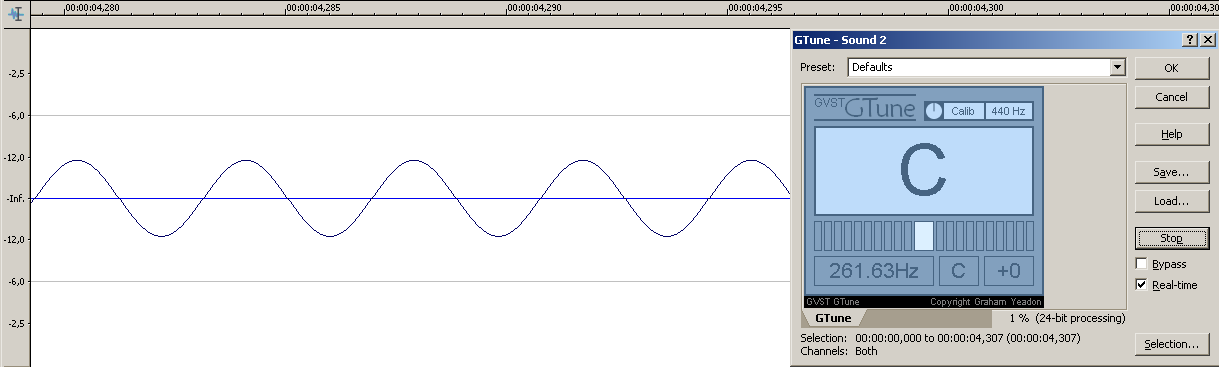
\includegraphics[width=17cm]{../img/png/testWaveGeneratorSinus.png}
\caption{Vérification des ondes générées grace à d'autres logiciels}
\end{figure}

Nos tests se contentent donc de générer un buffer, de le
sauvegarder, et renvoient un résultat à vrai.

\subsection{VCO}
Pour ce module, nous avons testé :
\begin{itemize}
    \item Qu'un onde  carrée demandée au wavegenerator se retrouvait bien dans le port d'entrée d'un module \textit{mock}. Ce test est effectué en mettant toutes les valeurs du buffer du mock dans un QSet et en constatant qu'au final, il ne contient que deux valeurs et que celles-ci sont opposées.
    \item Que la variation du k d'une unité faisait doubler la fréquence de l'onde obtenue.
    \item Que le sélecteur de forme d'onde sélectionnait effectivement l'onde demandée.
\end{itemize}

\subsection{VCA}
Le rôle du \verb!VCA! étant de multiplier chaque valeur de son entrée par un coeficient, son test a consisté à le faire fonctionner avec un gain donné et de vérifier que les valeurs produites dans un mock était conforme à nos attentes.

\subsection{VCF}

\subsubsection{Test VCF}

Le test du \verb!VCF! consiste à lier une instance de \verb!VCO! à
un \verb!VCF!. Le VCO ne produira qu'une onde de type \verb!Empty!,
donc ne produisant que des 0. Nous utilisons le filtre
\verb!FilterIncrement! qui se contente d'ajouter 1 à toute valeur
du buffer s'entrée si elle est positive, ou --1 si elle est
négative. Le test s'assure que le buffer de sortie du \verb!VCF! ne
contient que des 1.

\subsubsection{Les filtres}

Il n'est pas possible de tester simplement les filtres. Tout comme
pour les \verb!WaveGenerators!, il faudrait décomposer le signal
afin de tester son intégrité. Cependant, là où la génération
fournie par les \verb!WaveGenerators! pouvait être étudiée par la
suite sous des logiciels tels que Soundforge ou Audacity, il n'en
est pas de même pour les filtres. Nous avons donc décidé de se fier
à l'écoute du signal.

\subsection{Test ADSR}

Nous avons testé ce module grace au fait que son comportement soit lié à ce qu'il reçoit dans son port \texttt{gate}. Sur une \textit{durée} de trois buffers, nous lui envoyons donc des valeurs 1, puis des zeros, puis des 1, ce qui correspond à un cycle ADSR complet. Les résultats des \og{}process\fg{} sont stockés dans un buffer puis analysé par parcours dudit buffer à la recherche de chaque segment du cycle. Les quatres valeurs obtenues sont ensuité comparées à celles données en entrée.


\subsection{Test Mixer}

Le test du mixer est réalisé en plaçant des buffers constants en entrée de chaque\dots entrée et en constatant que le buffer de sortie est également constant avec pour valeur celle des entrée.


\subsection{Test WavRecorder}

Le test du \verb!WavRecorder! consiste à relier un \verb!VCO!
utilisant le \verb!WaveGeneratorSquare!, produisant une forme
d'onde carrée à periode fixe, à l'entrée du \verb!WavRecorder!,
dans un fichier donné, en précisant un nombre défini d'itérations
au \verb!WavRecorder! afin qu'il ferme le fichier de sortie au bout
de ces itérations.

Une fois l'enregistrement terminé, on ouvre le fichier en lecture,
puis on passe le header du fichier WAV, et l'on s'assure que l'on
ne trouve bien que deux valeurs différentes (front
montant/descendant) jusqu'à la fin du fichier.

\subsection{Test WavLooper}

Le test du \verb!WavLooper! consiste à charger un fichier
\verb!WAV! ne comportant que deux valeurs différentes, le faire
lire ce fichier, puis de vérifier que la sortie du buffer ne
comporte qu'une suite de deux valeurs.

\subsection{Test Sampler}
Pour effectuer et automatiser le test de ce module, nous utilisons sa capacité à être commandé par un port \texttt{gate}
. Le test consiste donc à faire fonctionner le module un nombre arbitraire de fois en lui donnant~: 
\begin{itemize}
    \item sur le port gate~: alternativement 0, 1 ou 2
    \item sur le port d'entrée, le buffer est rempli d'entier, chacun d'eux correspondant à sa place dans le buffer.
\end{itemize}
Le resultat attendu est alors~:
\begin{itemize}
    \item une période ou le sampler est inactif (gate = 0)
    \item une période d'enregistrement de l'entrée
    \item puis alternativement des périodes de lecture et de pause.
\end{itemize}

Le buffer de sortie est analysé à chaque pas du test, il doit être conforme aux attentes pour que le résultat du test reste valide.


\end{document}
